\appendix
\chapter{Appendix}

\section{Dependencies}
\label{sec:dependencies}

A complete list of python packages used for the implementation and experiments:

\begin{itemize}
    \item Babel version 2.9.1
    \item kmeans\_pytorch version 0.3
    \item matplotlib version 3.3.4
    \item numpy version 1.20.2
    \item pandas version 1.2.4
    \item Pillow version 8.2.0
    \item rsa version 4.7.2
    \item torch version 1.8.1
    \item torchvision version 0.9.1
\end{itemize}

\section{Additional figures}
\label{sec:appendix:additional-figures}
\subsection{Experiments for fine-tuning} \label{sec:appendix:finetuning-plots}
%%%%%%%%%%%%%%%%%%%%%%%%%%%%%%%%%%%%%%%%%%% MNIST models
\begin{figure}
     \centering
     \begin{subfigure}[b]{0.49\textwidth}
         \centering
         \includegraphics[width=\textwidth]{images/finetuning/finetuning_protecting_content_smalllr_thesis_lenet1.eps}
         \caption{LeNet-1}
         \label{fig:finetuning_lenet1_smalllr}
     \end{subfigure}
     \hfill
     \begin{subfigure}[b]{0.49\textwidth}
         \centering
         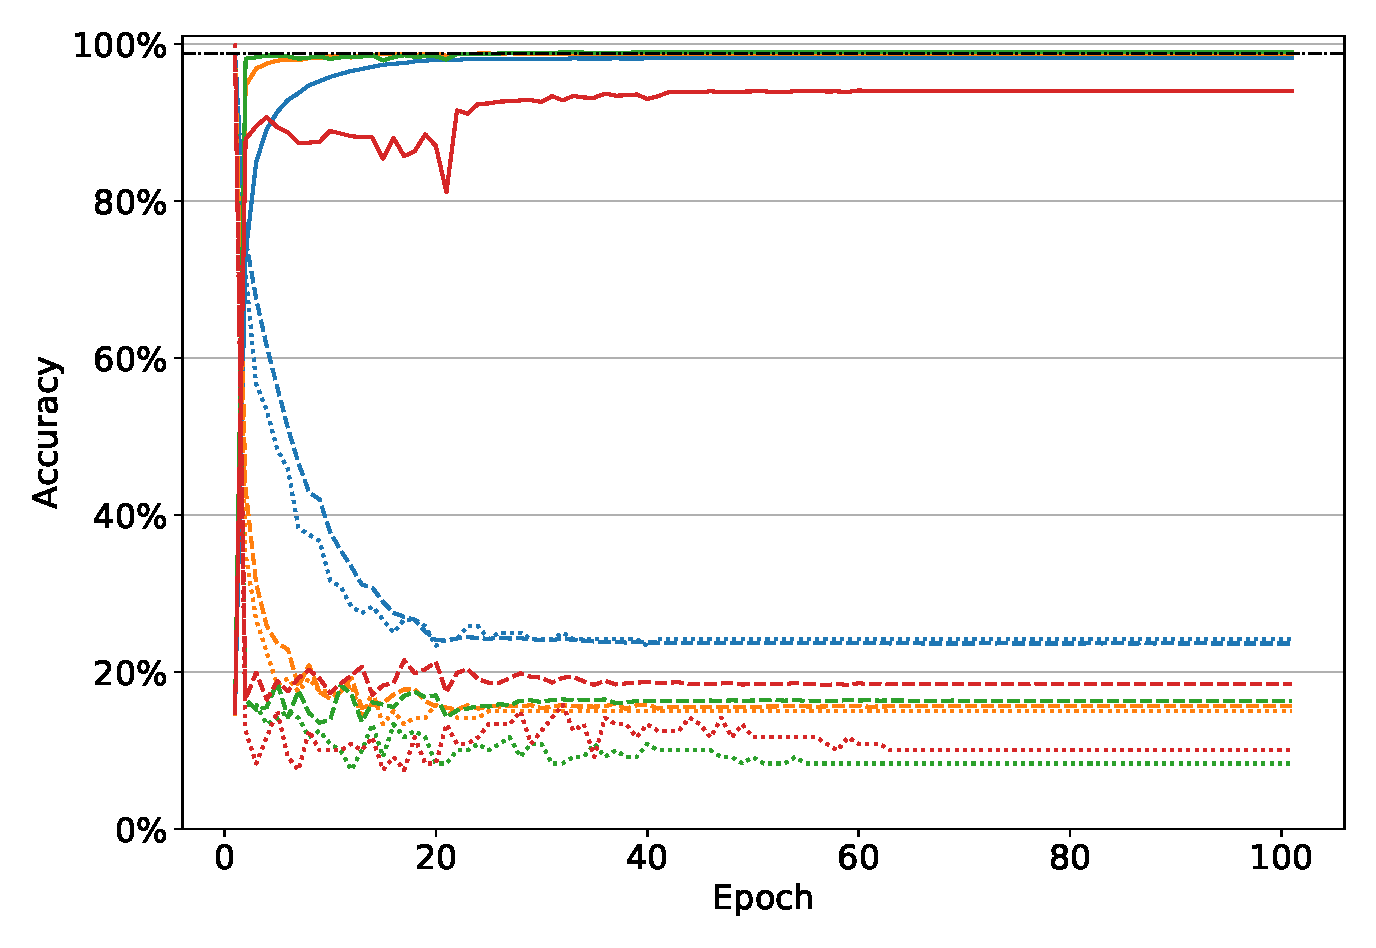
\includegraphics[width=\textwidth]{images/finetuning/finetuning_protecting_content_largelr_thesis_lenet1.eps}
         \caption{LeNet-1}
         \label{fig:finetuning_lenet1_largelr}
     \end{subfigure}
     \begin{subfigure}[b]{0.49\textwidth}
         \centering
         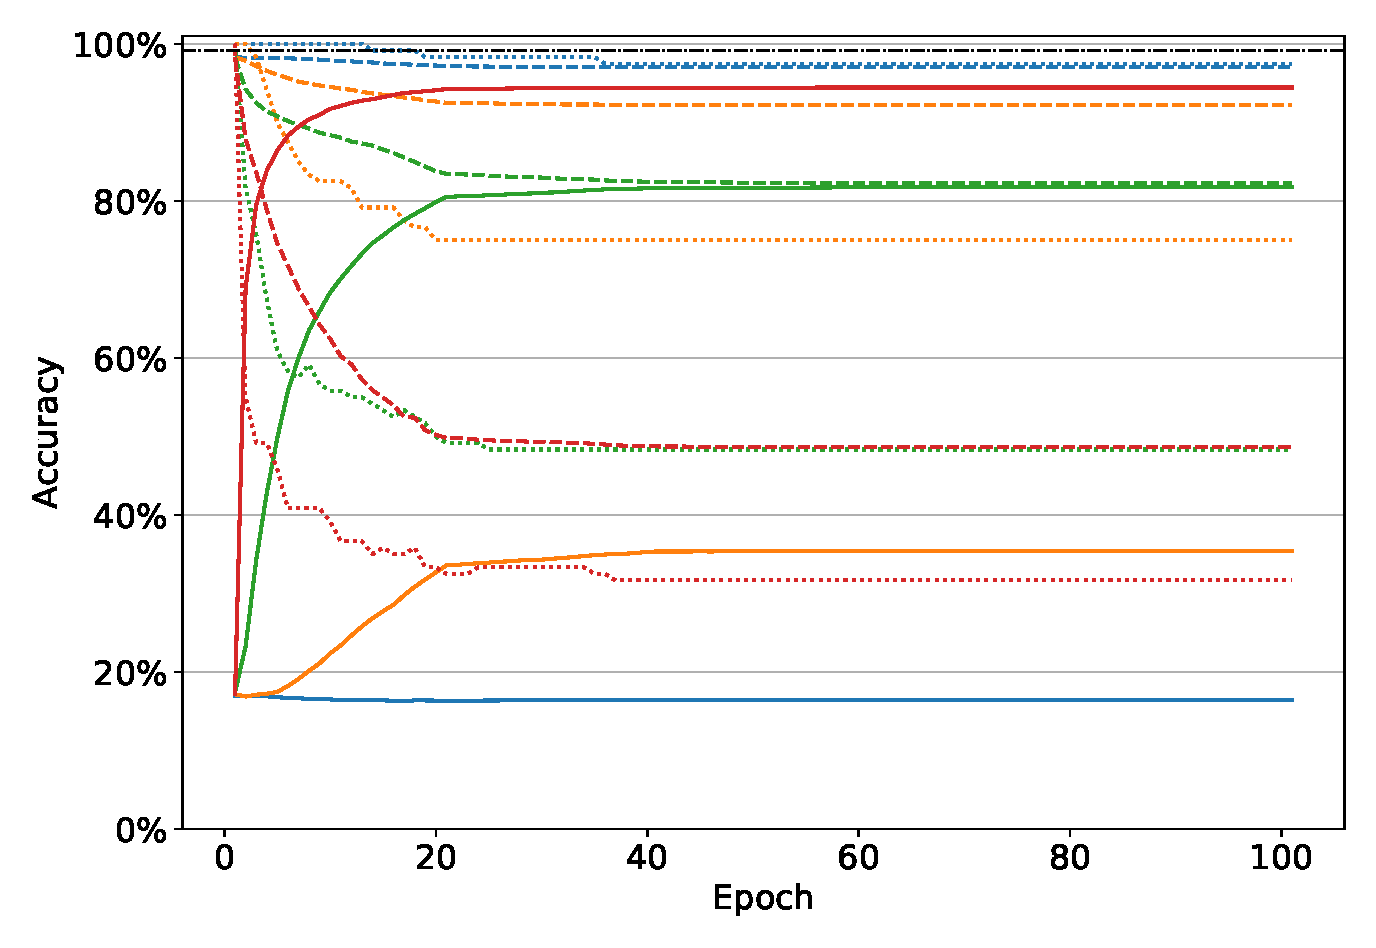
\includegraphics[width=\textwidth]{images/finetuning/finetuning_protecting_content_smalllr_thesis_lenet3.eps}
         \caption{LeNet-3}
         \label{fig:finetuning_lenet3_smalllr}
     \end{subfigure}
     \hfill
     \begin{subfigure}[b]{0.49\textwidth}
         \centering
         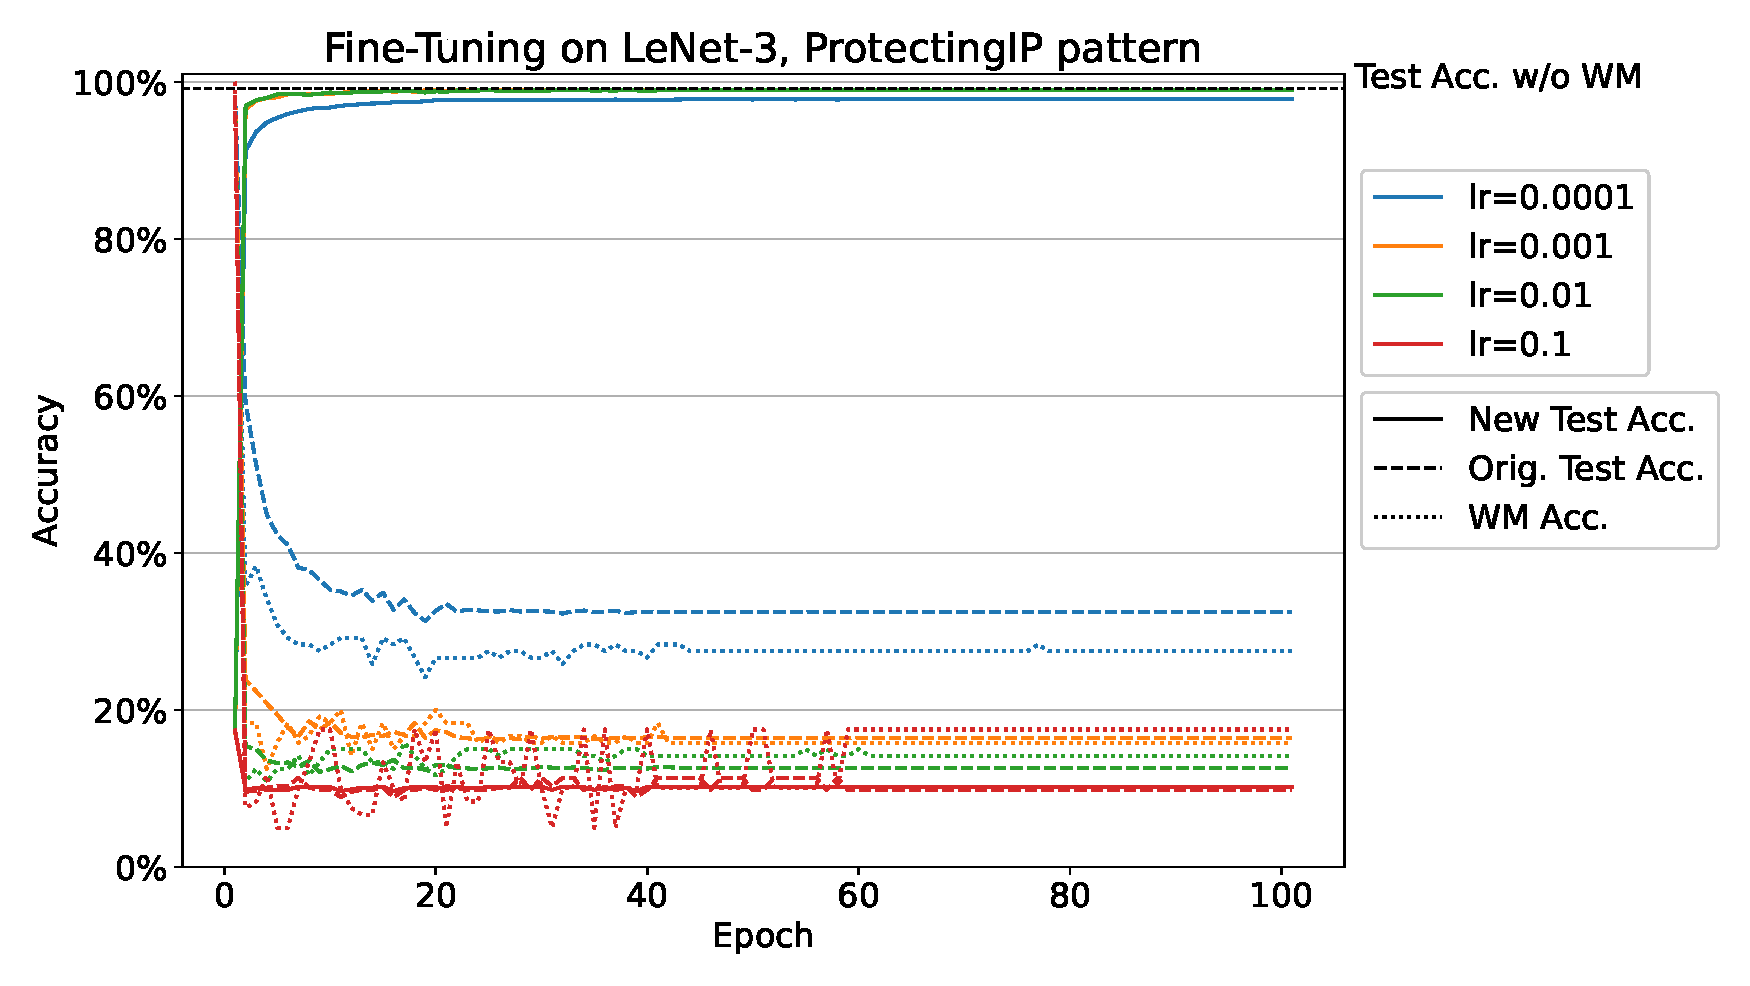
\includegraphics[width=\textwidth]{images/finetuning/finetuning_protecting_content_largelr_thesis_lenet3.eps}
         \caption{LeNet-3}
         \label{fig:finetuning_lenet3_largelr}
     \end{subfigure}
     \hfill
     \begin{subfigure}[b]{0.49\textwidth}
         \centering
         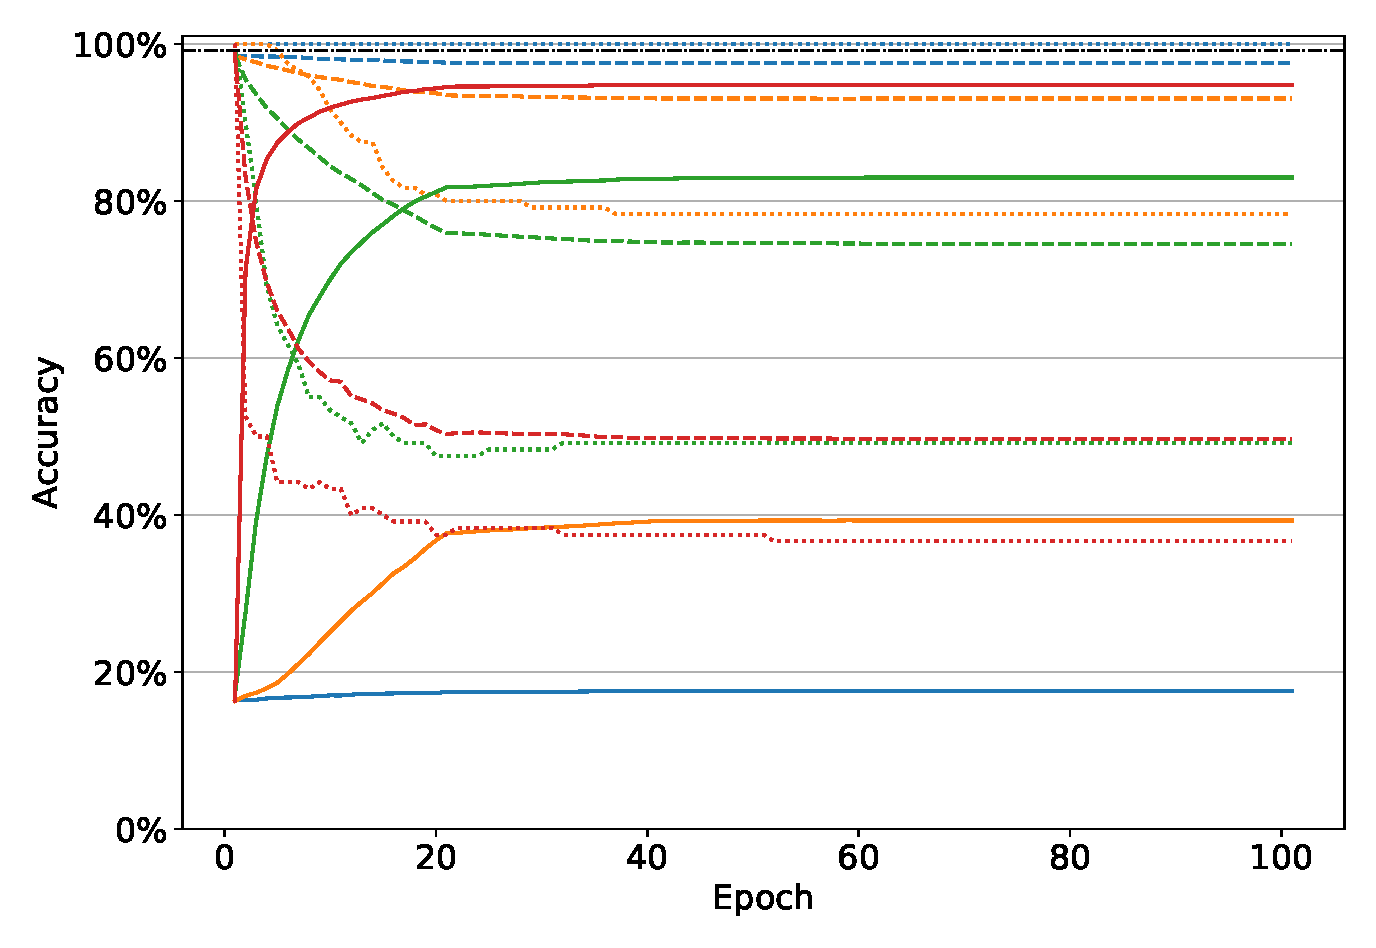
\includegraphics[width=\textwidth]{images/finetuning/finetuning_protecting_content_smalllr_thesis_lenet5.eps}
         \caption{LeNet-5}
         \label{fig:finetuning_lenet5_smalllr}
     \end{subfigure}
     \hfill
     \begin{subfigure}[b]{0.49\textwidth}
         \centering
         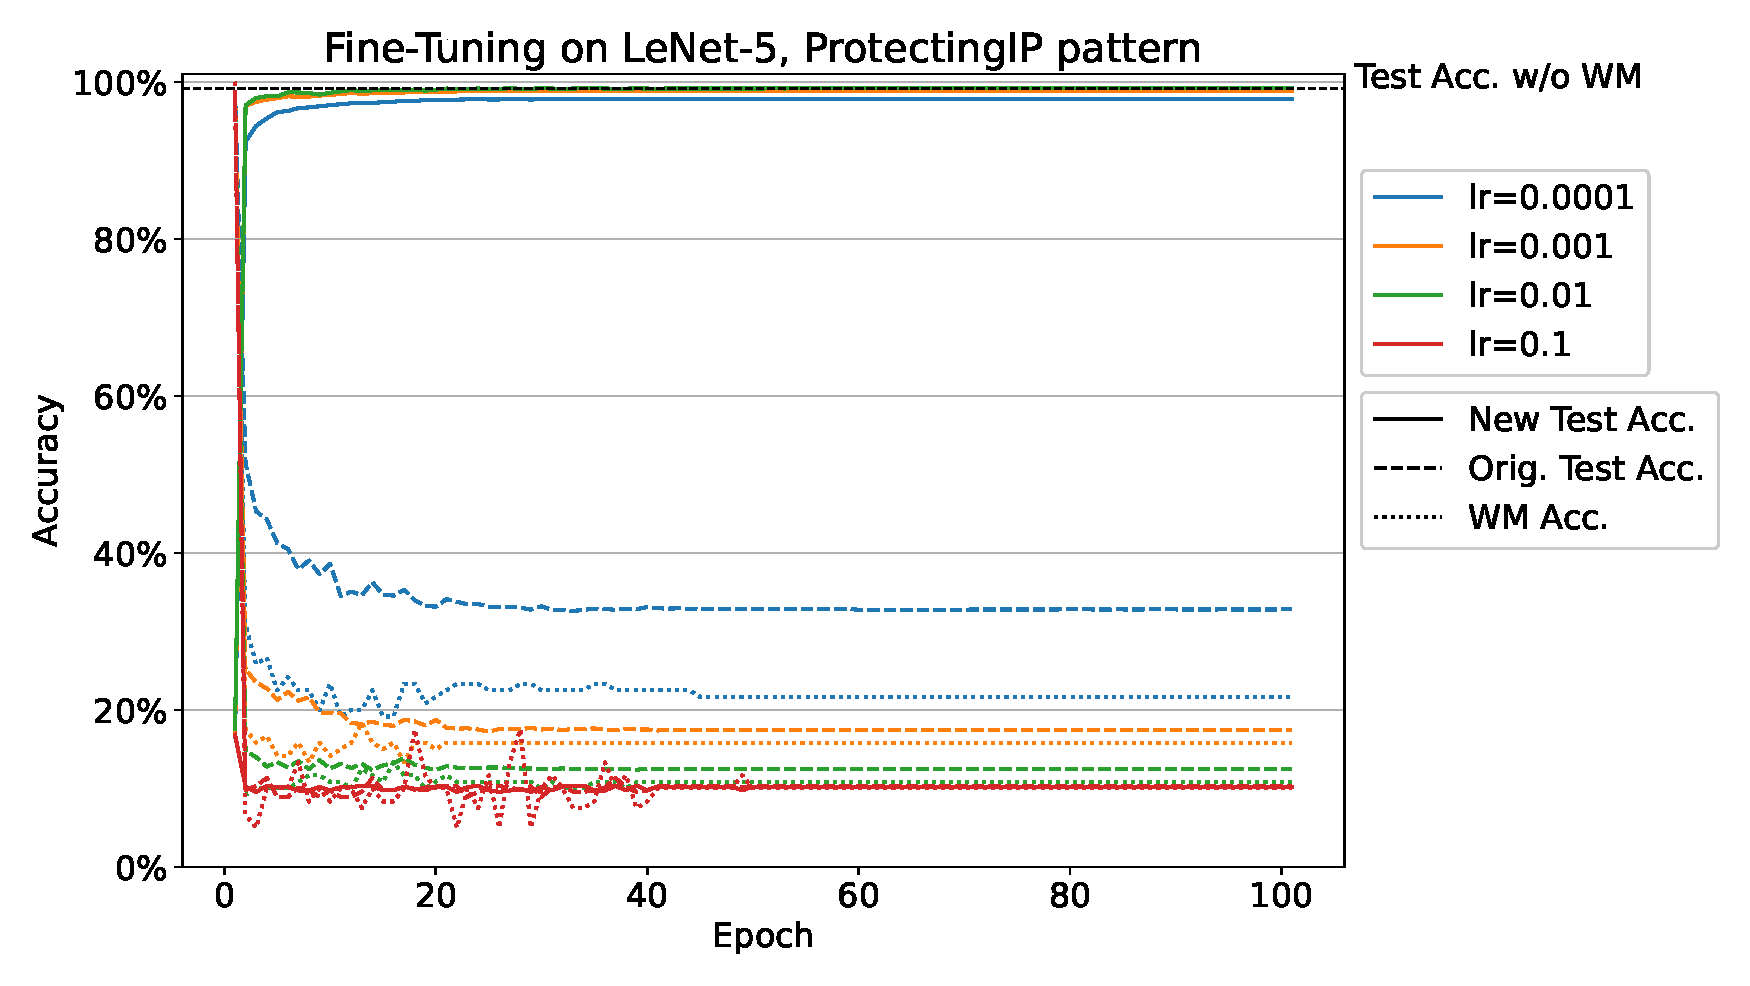
\includegraphics[width=\textwidth]{images/finetuning/finetuning_protecting_content_largelr_thesis_lenet5.eps}
         \caption{LeNet-5}
         \label{fig:finetuning_lenet5_largelr}
     \end{subfigure}
     \hfill
     
     \begin{subfigure}[b]{\textwidth}
         \centering
         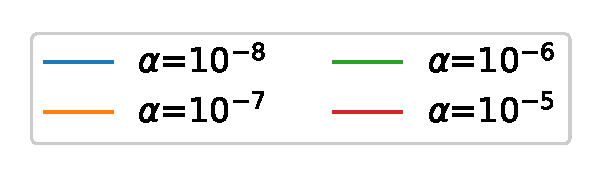
\includegraphics[height=1.1cm]{images/finetuning/legend_content_finetuning_smalllr_colors.eps}
         \quad
         \includegraphics[height=1.3cm]{images/finetuning/legend_content_finetuning_linetypes.eps}
         \quad
         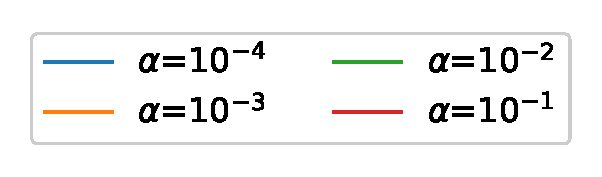
\includegraphics[height=1.1cm]{images/finetuning/legend_content_finetuning_largelr_colors.eps}
     \end{subfigure}
     
     \caption{Fine-tuning on \textbf{MNIST} models, watermarked with \textit{ProtectingIP-pattern}. The plots on the left side correspond to fine-tuning with smaller learning rates and the ones on the right side to fine-tuning with larger learning rates. The black dash-dotted line corresponds to the benchmark test accuracy of the non-watermarked model.}
     \label{fig:finetuning_mnistmodels}
\end{figure}

%%%%%%%%%%%%%%%%%%%%%%%%%%%%%%%%%%%%%%%%%%% CIFAR-10

\begin{figure}
     \centering
     \begin{subfigure}[b]{0.49\textwidth}
         \centering
         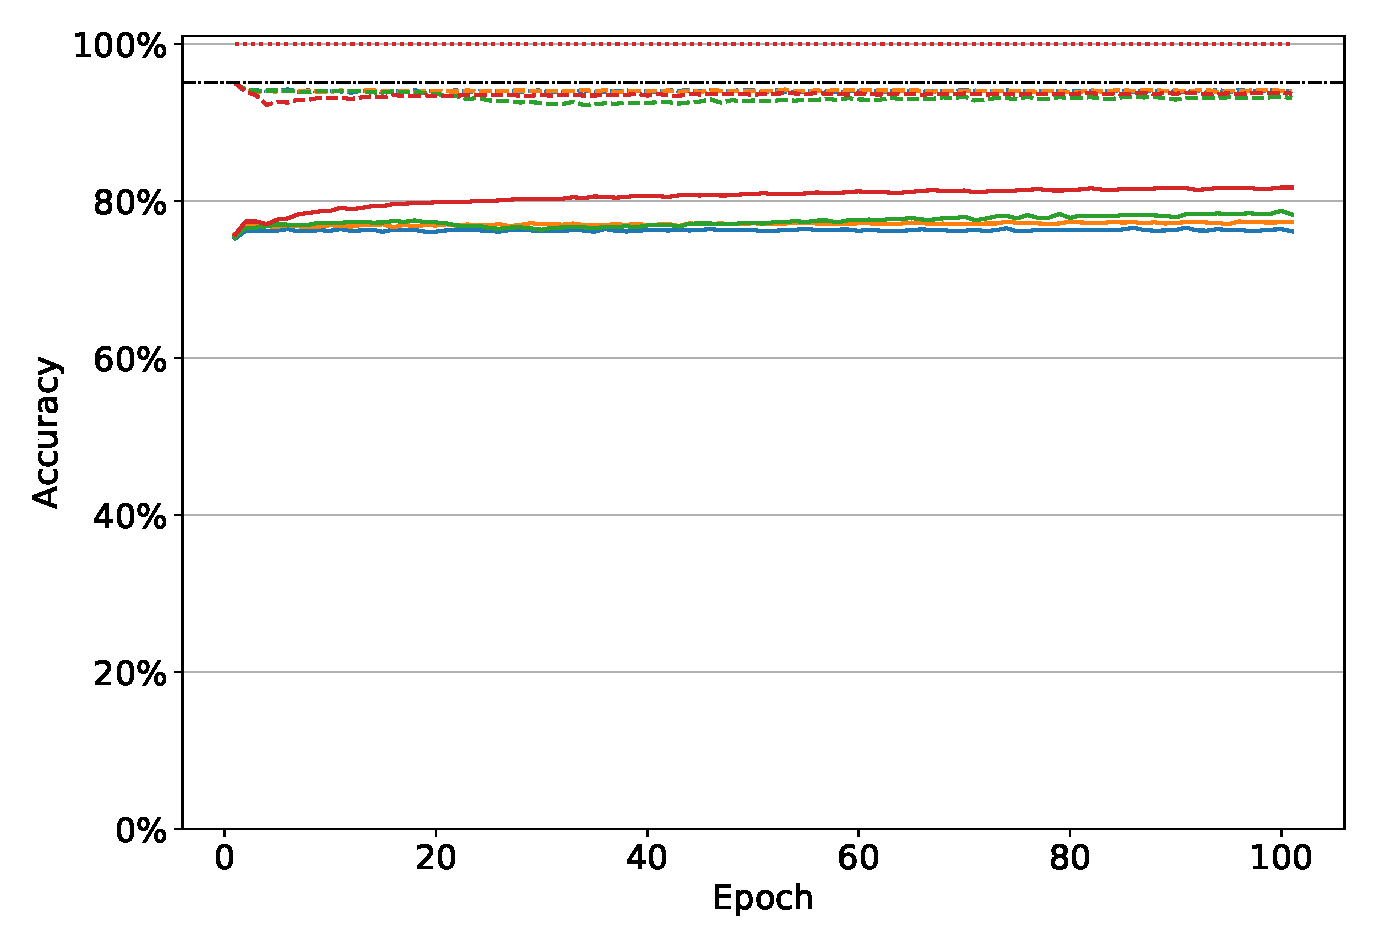
\includegraphics[width=\textwidth]{images/finetuning/finetuning_protecting_content_smalllr_thesis_resnet18.eps}
         \caption{ResNet-18}
         \label{fig:finetuning_resnet18_smalllr}
     \end{subfigure}
     \hfill
     \begin{subfigure}[b]{0.49\textwidth}
         \centering
         \includegraphics[width=\textwidth]{images/finetuning/finetuning_protecting_content_largelr_thesis_resnet18.eps}
         \caption{ResNet-18}
         \label{fig:finetuning_resnet18_largelr}
     \end{subfigure}
     \begin{subfigure}[b]{0.49\textwidth}
         \centering
         \includegraphics[width=\textwidth]{images/finetuning/finetuning_protecting_content_smalllr_thesis_resnet34.eps}
         \caption{ResNet-34}
         \label{fig:finetuning_resnet34_smalllr}
     \end{subfigure}
     \hfill
     \begin{subfigure}[b]{0.49\textwidth}
         \centering
         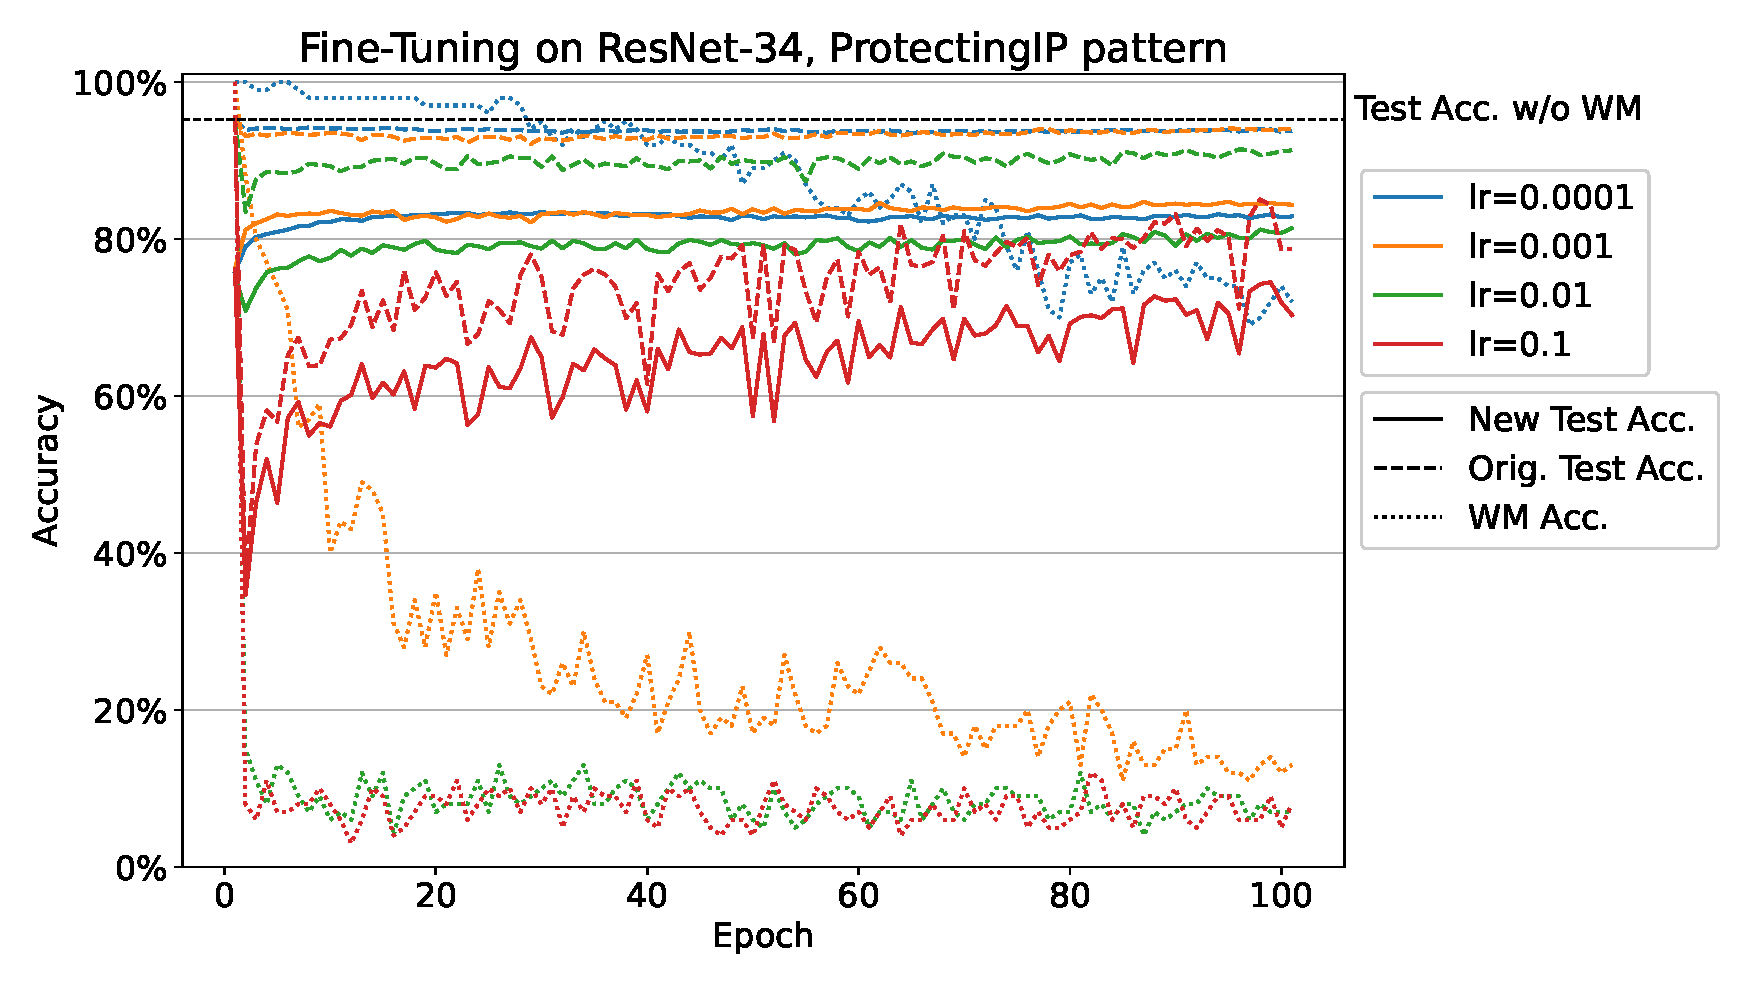
\includegraphics[width=\textwidth]{images/finetuning/finetuning_protecting_content_largelr_thesis_resnet34.eps}
         \caption{ResNet-34}
         \label{fig:finetuning_resnet34_largelr}
     \end{subfigure}
     \hfill
     \begin{subfigure}[b]{0.49\textwidth}
         \centering
         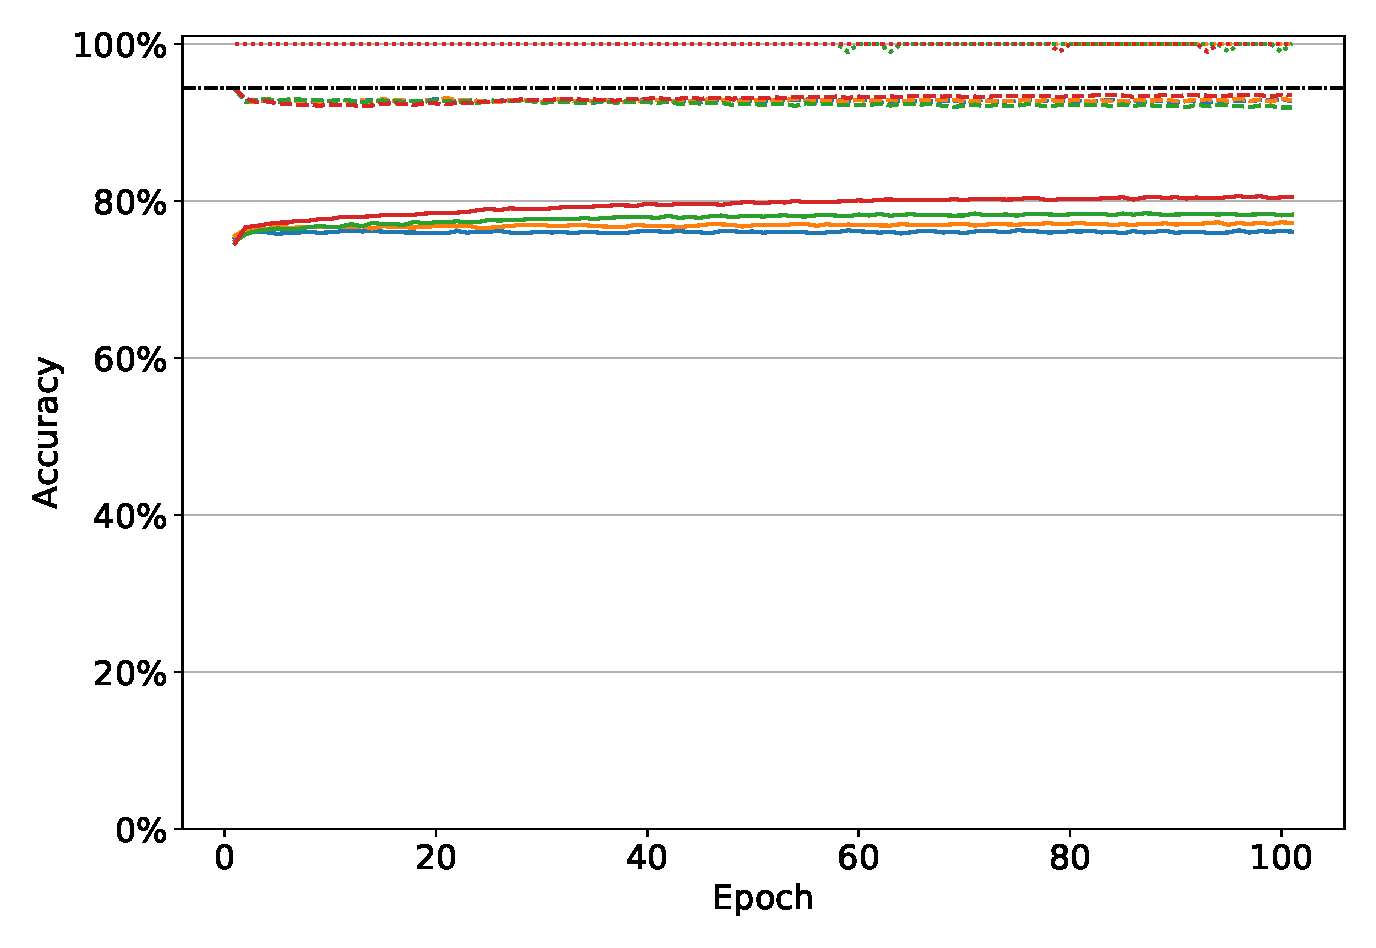
\includegraphics[width=\textwidth]{images/finetuning/finetuning_protecting_content_smalllr_thesis_resnet50.eps}
         \caption{ResNet-50}
         \label{fig:finetuning_resnet50_smalllr}
     \end{subfigure}
     \hfill
     \begin{subfigure}[b]{0.49\textwidth}
         \centering
         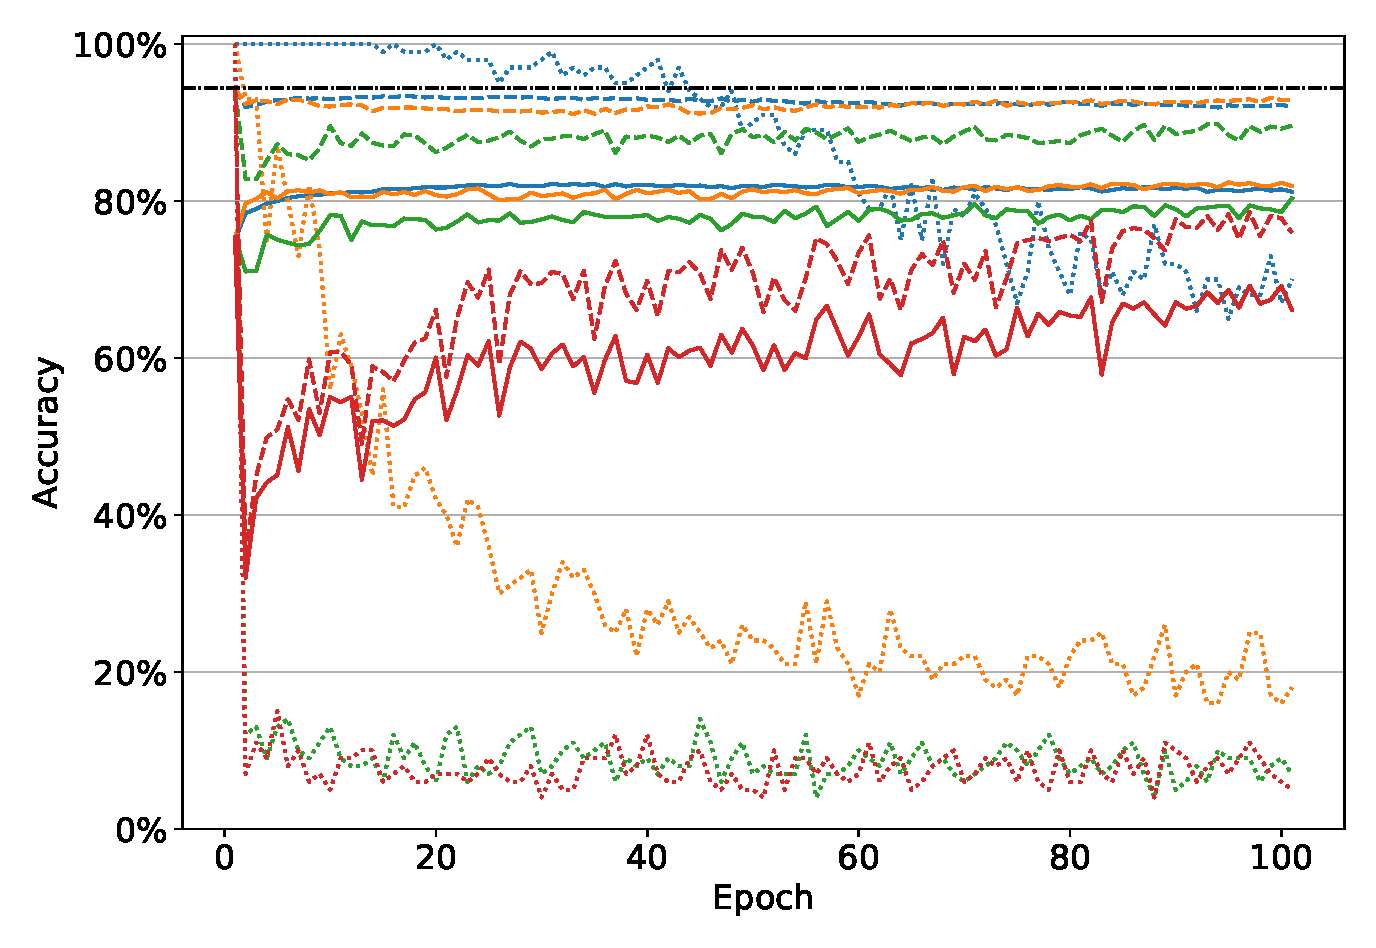
\includegraphics[width=\textwidth]{images/finetuning/finetuning_protecting_content_largelr_thesis_resnet50.eps}
         \caption{ResNet-50}
         \label{fig:finetuning_resnet50_largelr}
     \end{subfigure}
     \hfill
     
     \begin{subfigure}[b]{\textwidth}
         \centering
         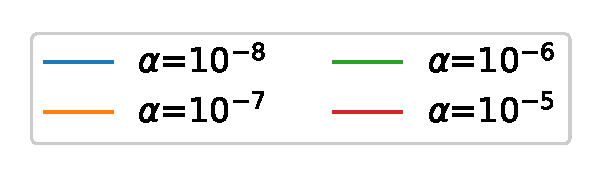
\includegraphics[height=1cm]{images/finetuning/legend_content_finetuning_smalllr_colors.eps}
         \quad
         \includegraphics[height=1.3cm]{images/finetuning/legend_content_finetuning_linetypes.eps}
         \quad
         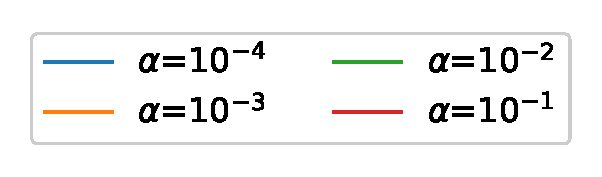
\includegraphics[height=1cm]{images/finetuning/legend_content_finetuning_largelr_colors.eps}
     \end{subfigure}
     
     \caption{Fine-tuning on \textbf{CIFAR-10} models, watermarked with \textit{ProtectingIP-pattern}. The plots on the left side correspond to fine-tuning with smaller learning rates and the ones on the right side to fine-tuning with larger learning rates. The black dash-dotted line corresponds to the benchmark test accuracy of the non-watermarked model.}
     \label{fig:finetuning_cifar10models}
\end{figure}


\begin{figure}
\centering
\begin{subfigure}[b]{0.49\textwidth}
    \centering
    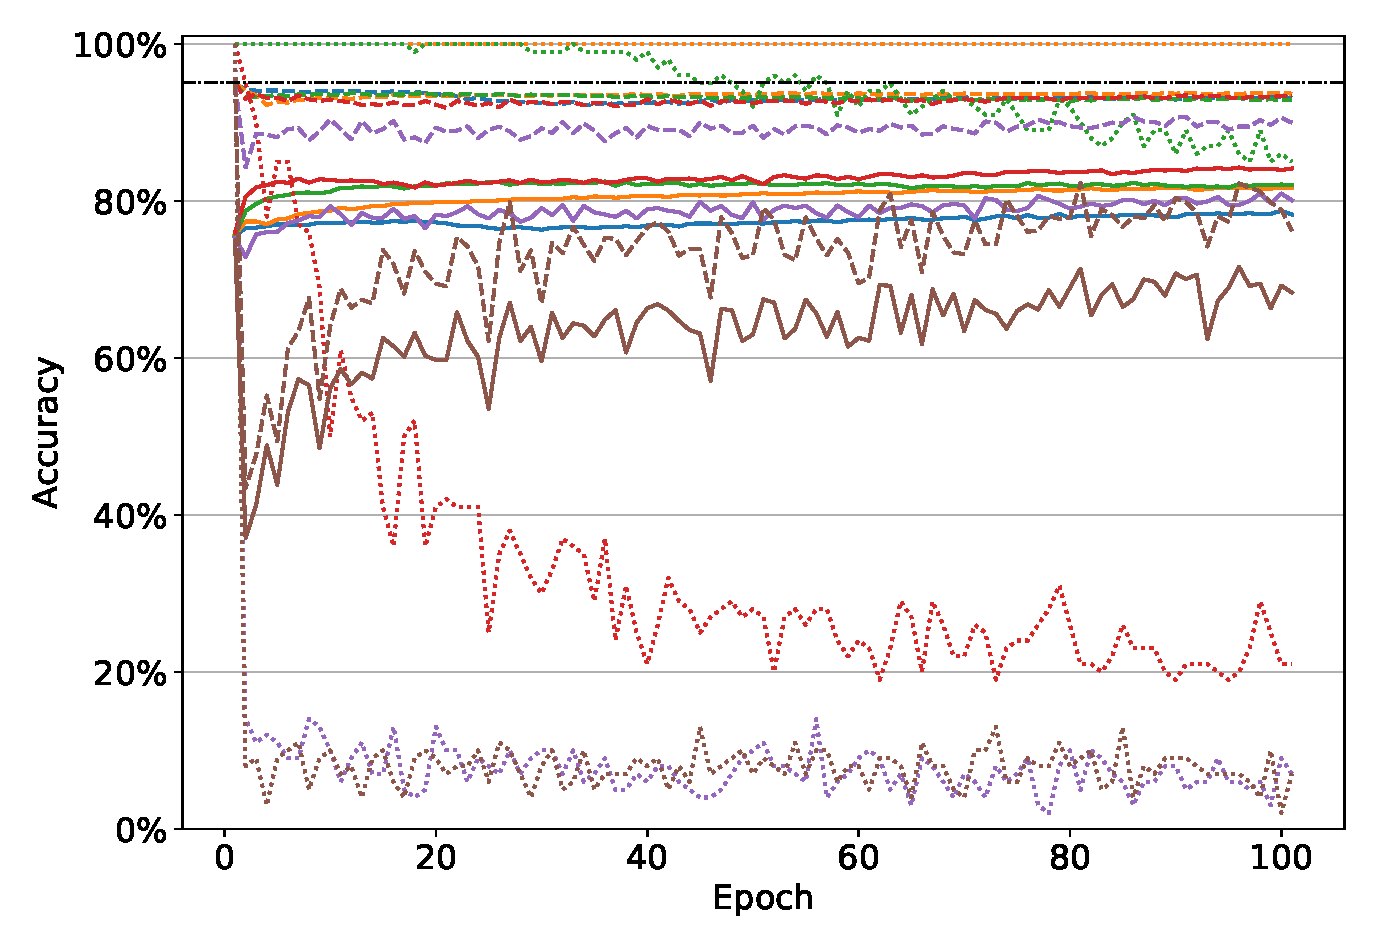
\includegraphics[width=\linewidth]{images/finetuning/finetuning_protecting_content_imagenet_0.eps}
    \caption{Fine-Tuning on CINIC-10}
\end{subfigure}
\begin{subfigure}[b]{0.49\textwidth}
    \centering
    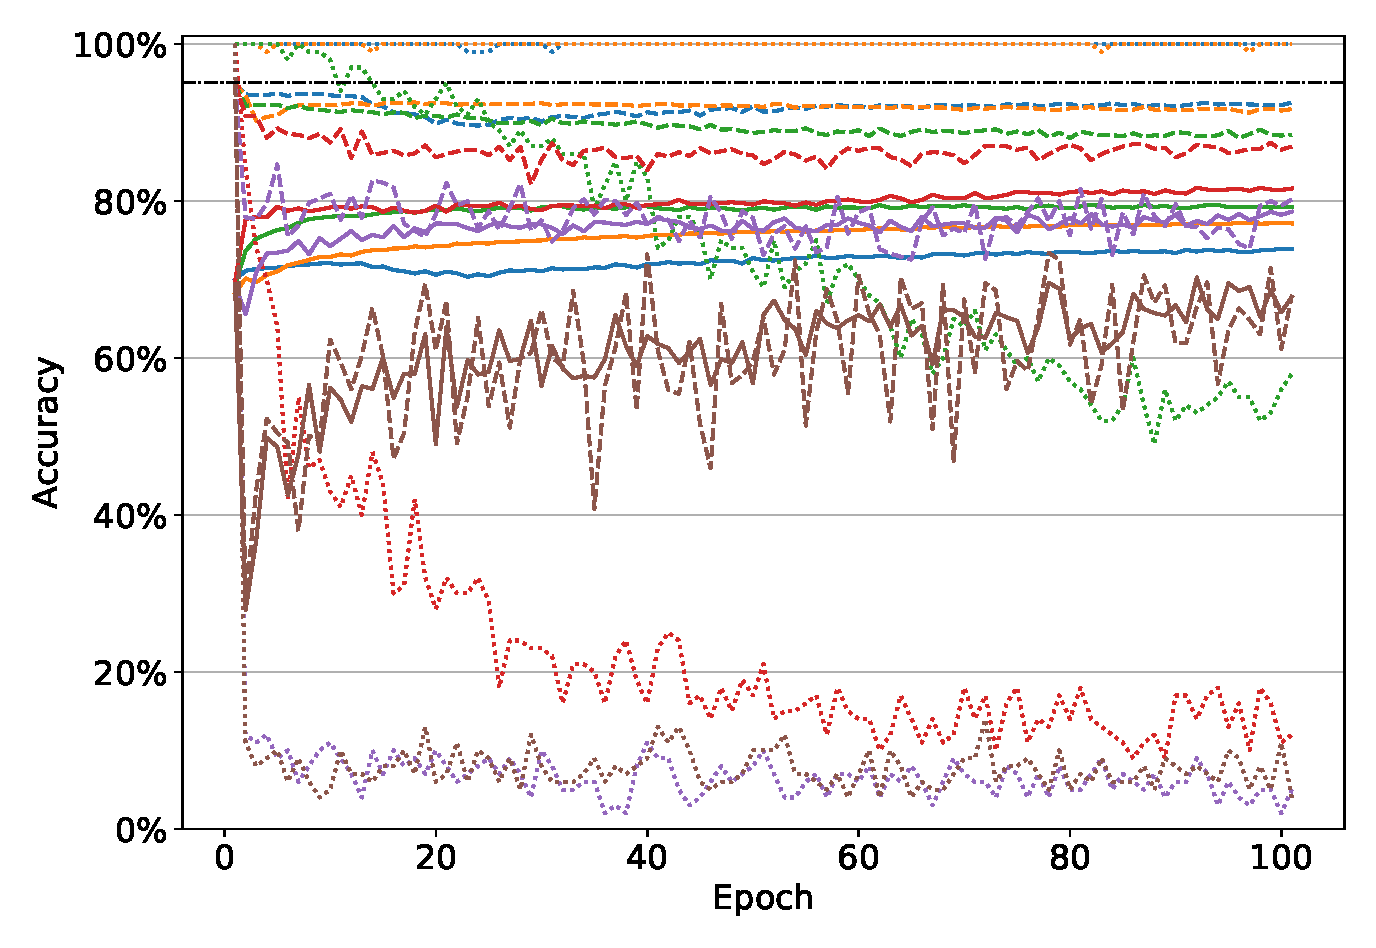
\includegraphics[width=\linewidth]{images/finetuning/finetuning_protecting_content_imagenet_1.eps}
    \caption{Fine-Tuning on ImageNet part of CINIC-10}
\end{subfigure}

\begin{subfigure}[b]{\linewidth}
    \centering
    \includegraphics[height=1.1cm]{images/finetuning/legend_content_finetuning_imagenet_colors.eps}
    \quad
    \includegraphics[height=1.1cm]{images/finetuning/legend_content_finetuning_imagenet_linetypes.eps}
\end{subfigure}

\caption{Fine-Tuning on both, CINIC-10 and only on the ImageNet part of CINIC-10. Original line plots to \cref{fig:fine-tuning-both-cinic10-imagenet}.}
\label{fig:fine-tuning-both-cinic10-imagenet-original}

\end{figure}
%\clearpage
%\section{Results for plots}
%\begin{table}
\centering
\small
\caption{Additional experiments for \textit{FrontierStitching}, varying $\epsilon$: fidelity}
\label{tab:results_frontier_fidelity}
\begin{tabular}{|l|l|l||l|l|l|}
\hline
\multicolumn{3}{|c|}{\textbf{CIFAR-10}}     & \multicolumn{3}{c|}{\textbf{MNIST}}         \\ \hline
Arch      & $\epsilon$    & Rel. valid. loss diff. & Arch      & $\epsilon$    & Rel. valid. loss diff. \\ \hline
DenseNet  & 0.0001 & 0.2342                 & SimpleNet & 0.0001 & 0.1551                 \\ \hline
          & 0.001  & 0.3298                 &           & 0.001  & 0.0785                 \\ \hline
          & 0.01   & 0.289                  &           & 0.01   & 0.1363                 \\ \hline
          & 0.1    & 0.3605                 &           & 0.1    & 0.1184                 \\ \hline
          & 0.25   & 0.3394                 &           & 0.25   & 0.144                  \\ \hline
          & 0.5    & 0.2996                 &           & 0.5    & 0.1635                 \\ \hline
          & 1      & 0.3394                 &           & 1      & 0.0776                 \\ \hline
ResNet-18 & 0.0001 & 0.1966                 & LeNet-1   & 0.0001 & 1.0639                 \\ \hline
          & 0.001  & 0.1521                 &           & 0.001  & 1.1265                 \\ \hline
          & 0.01   & 0.1837                 &           & 0.01   & 0.5238                 \\ \hline
          & 0.1    & 0.1739                 &           & 0.1    & 0.4911                 \\ \hline
          & 0.25   & 0.1441                 &           & 0.25   & 0.4376                 \\ \hline
          & 0.5    & 0.095                  &           & 0.5    & 0.0765                 \\ \hline
          & 1      & 0.1378                 &           & 1      & 0.013                  \\ \hline
ResNet-34 & 0.0001 & 0.0689                 & LeNet-3   & 0.0001 & 1.3487                 \\ \hline
          & 0.001  & 0.1154                 &           & 0.001  & 1.2401                 \\ \hline
          & 0.01   & 0.0844                 &           & 0.01   & 1.3268                 \\ \hline
          & 0.1    & 0.0311                 &           & 0.1    & 0.6569                 \\ \hline
          & 0.25   & 0.0815                 &           & 0.25   & 0.7123                 \\ \hline
          & 0.5    & 0.1141                 &           & 0.5    & 0.285                  \\ \hline
          & 1      & 0.0906                 &           & 1      & 0.127                  \\ \hline
ResNet-50 & 0.0001 & 0.0463                 & LeNet-5   & 0.0001 & 1.0773                 \\ \hline
          & 0.001  & 0.1331                 &           & 0.001  & 1.1608                 \\ \hline
          & 0.01   & 0.1566                 &           & 0.01   & 1.2101                 \\ \hline
          & 0.1    & 0.0892                 &           & 0.1    & 0.7567                 \\ \hline
          & 0.25   & 0.0971                 &           & 0.25   & 0.5123                 \\ \hline
          & 0.5    & 0.1807                 &           & 0.5    & 0.3898                 \\ \hline
          & 1      & 0.2041                 &           & 1      & 0.1825                 \\ \hline
\end{tabular}
\end{table}
%\input{tables/tab-results_frontier_pruning}